%%%%%%%%%%%%%%%
\begin{frame}{}
  \begin{exampleblock}{SM Problem $14.44$: Consistent Enumerations}
    Suppose the following are three consistent enumerations of an ordered set $A = \set{a, b, c, d}$:
    \begin{align*}
      A_1: \quad a \qquad \red{b} \qquad \red{c} \qquad d \\
      A_2: \quad a \qquad c \qquad b \qquad d \\
      A_3: \quad a \qquad c \qquad \blue{d} \qquad \blue{b}
    \end{align*}
    Assuming the Hasse diagram $D$ of $A$ is \purple{connected}, draw $D$.
  \end{exampleblock}

  \pause
  \[
    b \prec_{A_1} c \land c \prec_{A_2} b \implies b \parallel_{A} c
  \]

  \[
    d \prec_{A_3} b \land b \prec_{A_2} d \implies b \parallel_{A} d
  \]
\end{frame}
%%%%%%%%%%%%%%%

%%%%%%%%%%%%%%%
\begin{frame}{}
  \fig{width = 0.25\textwidth}{figs/poset-abcd-hasse}

  \hrule
  \begin{columns}[t]
    \pause
    \column{0.50\textwidth}
      \fig{width = 0.50\textwidth}{figs/poset-abcd-hasse-2}
      \pause
      \[
	\purple{\# = 6}
      \]
    \pause
    \column{0.50\textwidth}
      \fig{width = 0.50\textwidth}{figs/poset-abcd-hasse-1}
      \pause
      \[
	\purple{\# = 3}
      \]
  \end{columns}
\end{frame}
%%%%%%%%%%%%%%%

%%%%%%%%%%%%%%%
\begin{frame}{}
  \begin{figure}
    \centering
    \resizebox{0.90\textwidth}{!}{% chain-intersection.tex

\begin{tikzpicture}[node distance = 0.00cm]
  \node (abcd) [] {
\includegraphics[scale = 0.30]{figs/chain-abcd}};
  \uncover<2->{\node (cap1) [red, right = of abcd] {$\cap$};}
  \node (acbd) [right = of cap1] {
\includegraphics[scale = 0.30]{figs/chain-acbd}};
  \uncover<2->{\node (cap2) [red, right = of acbd] {$\cap$};}
  \node (acdb) [right = of cap2] {
\includegraphics[scale = 0.30]{figs/chain-acdb}};

  \node (eq) [purple, right = of acdb] {$=$};
  \node (poset-abcd-hasse-1) [right = of eq] {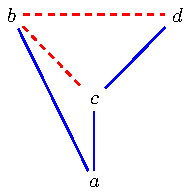
\includegraphics[scale = 0.40]{figs/poset-abcd-hasse-1}};
\end{tikzpicture}
}
  \end{figure}

  \uncover<3->{
    \begin{theorem}
      Every partial ordering on a set $X$ is the \red{intersection}
      of the total orders on $X$ \blue{containing it}.
    \end{theorem}
  }
\end{frame}
%%%%%%%%%%%%%%%